% !TEX TS-program = pdflatex
% !TEX encoding = UTF-8 Unicode

% This file is a template using the "beamer" package to create slides for a talk or presentation
% - Giving a talk on some subject.
% - The talk is between 15min and 45min long.
% - Style is ornate.

% MODIFIED by Jonathan Kew, 2008-07-06
% The header comments and encoding in this file were modified for inclusion with TeXworks.
% The content is otherwise unchanged from the original distributed with the beamer package.

\documentclass{beamer}

\mode<presentation>
{
  \usetheme{Malmoe}
  % or ...

  %\setbeamercovered{transparent}
  % or whatever (possibly just delete it)
}


\usepackage[english]{babel}
\usepackage{graphicx}
\usepackage{amssymb}
\usepackage{multicol,multirow,array}
\setbeamertemplate{navigation symbols}{}%remove navigation symbols
\setbeamertemplate{footline}[frame number]


\title[Association Testing with X Chromosome Data] % (optional, use only with long paper titles)
{Association Testing with X Chromosome Data\\
An Application To HCHS/SoL}

%\subtitle
%{Presentation Subtitle} % (optional)

\author[Caitlin McHugh, with Tim Thornton] % (optional, use only with lots of authors)
{Caitlin McHugh, with Tim Thornton}
% - Use the \inst{?} command only if the authors have different
%   affiliation.

\institute[University of Washington] % (optional, but mostly needed)
{
  Department of Biostatistics\\
  University of Washington
}
% - Use the \inst command only if there are several affiliations.
% - Keep it simple, no one is interested in your street address.

\date[Short Occasion] % (optional)
{26 Jan 2015}

% If you have a file called "university-logo-filename.xxx", where xxx
% is a graphic format that can be processed by latex or pdflatex,
% resp., then you can add a logo as follows:

% \pgfdeclareimage[height=0.5cm]{university-logo}{university-logo-filename}
% \logo{\pgfuseimage{university-logo}}

% If you wish to uncover everything in a step-wise fashion, uncomment
% the following command: 

%\beamerdefaultoverlayspecification{<+->}


\begin{document}

\begin{frame}
  \titlepage
\end{frame}

\begin{frame}{Outline}
 \tableofcontents
  % You might wish to add the option [pausesections]
\end{frame}

% Anything you have relevant to the "right" way to do association on the X chromosome in OLGA

\section{Intro}
\begin{frame}%{A Usual Test for Association}
\begin{itemize}
\item For each genotyped \textit{autosomal} SNP, we can fit a model of the form
$$ Y = \beta_0 + \beta_1 \mbox{SNP} + g_A + \mbox{covariates} +\epsilon$$ where
$$ g_A \sim MVN(0,\sigma_A^2 \mathbf{\Phi_A})$$
$$ \epsilon \sim MVN(0,\sigma_\epsilon^2 \mathbb{I})$$
\item When testing association on X chromosome SNPs, we propose to fit the model
$$ Y = \beta_0 + \beta_1 \mbox{SNP}_X + g_A + g_X + \mbox{covariates} +\epsilon$$ where further
$$ g_X \sim MVN(0,\sigma_X^2 \mathbf{\Phi_X})$$
\end{itemize}
% g_x and g_a are terms to adjust for background polygenic effects due to the autosomes and x chr
% we want to fit these terms separately since we've proven genetics on the autosome and x chr are different
\end{frame}

\section{Step 1: Estimate $\mathbf{\Phi_X}$}
\begin{frame}
\begin{itemize}
%\item We will call the X chromosome kinship matrix `$\mathbf{\Phi_X}$.'
\item The X chromosome kinship coefficient between individuals $i$ and $j$, $\Phi^X_{ij}$,  is defined as the probability of sampling one allele IBD at random from individual $i$ and individual $j$ on the X chromosome.
\item \textit{Note} for males there is no randomness in sampling, as there is only one allele at each location on the X chromosome.
\end{itemize}
\end{frame}

\begin{frame}
\begin{columns}
    \begin{column}{0.3\textwidth}
      \centering
      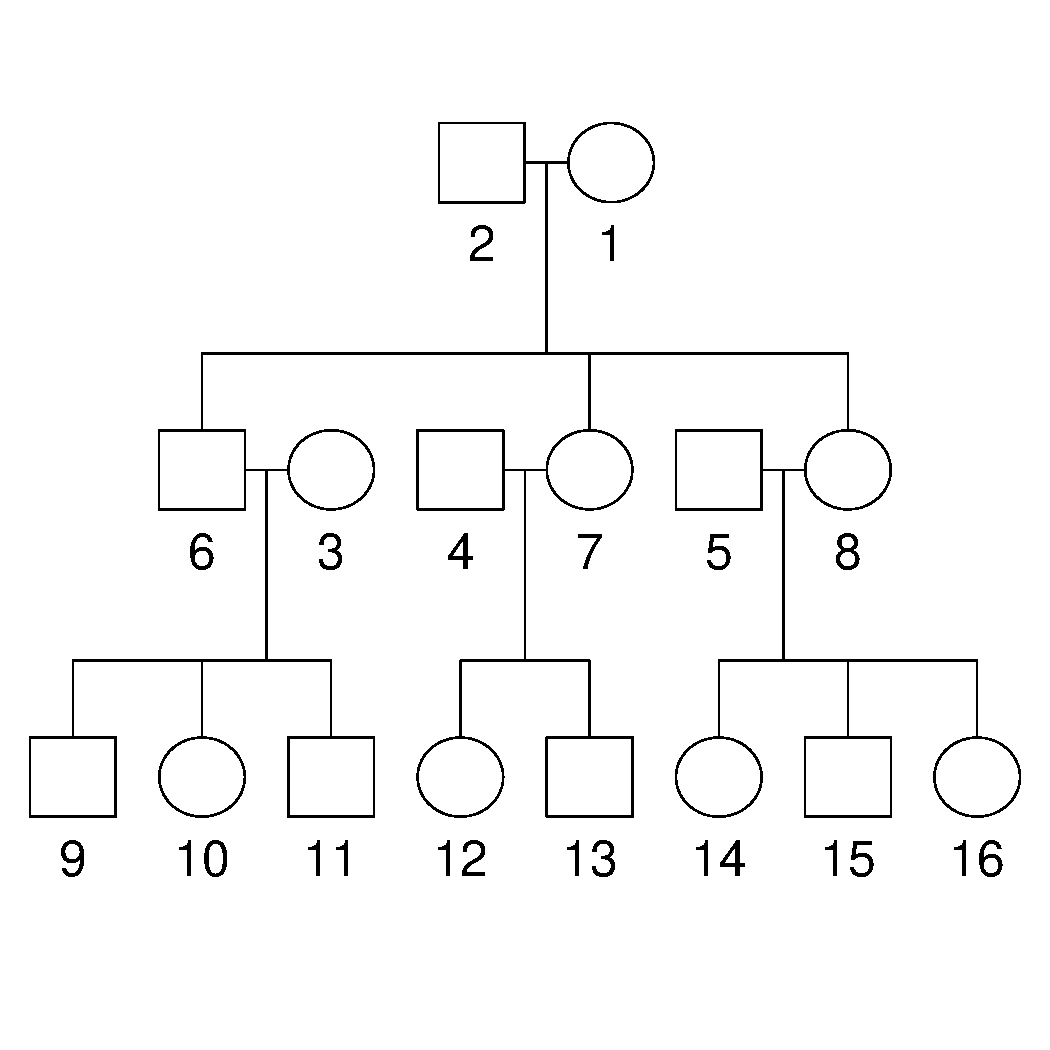
\includegraphics[height=4.5cm]{../pedigree_16individs.pdf}
    \end{column}
    \begin{column}{0.5\textwidth}
      \centering
      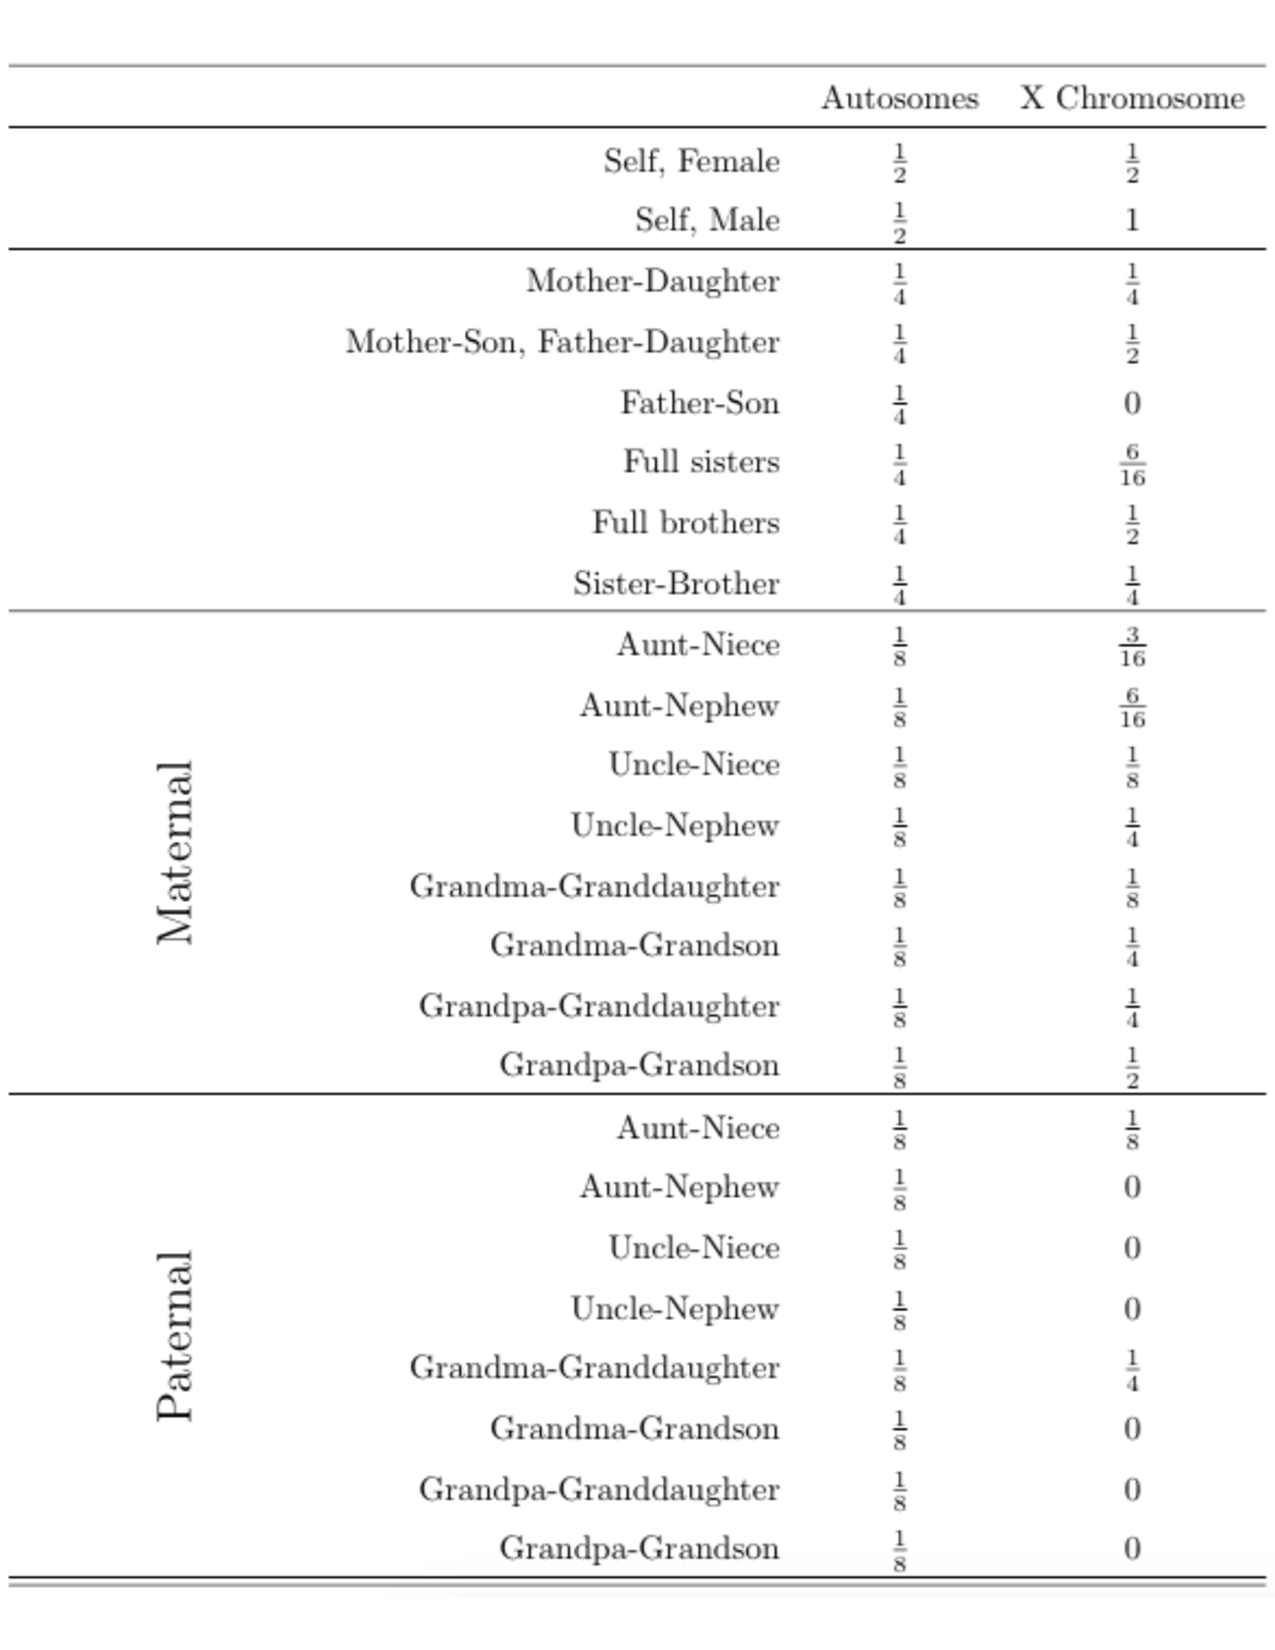
\includegraphics[height=8.3cm]{xchr_kc_values.pdf}
    \end{column}
 \end{columns}
\end{frame}

\begin{frame}
%\frametitle{Step 1: Estimate $\Phi_X$}
\begin{itemize}
%\item We assume a total of $N$ X chromosome SNPs; males coded 0, 2 and females coded 0, 1, 2.
\item We can estimate $\mathbf{\Phi_X}$ using the following GRM equations:
\begin{align*}
\mbox{GR}_{FF}&=\frac{1}{N}\sum_{i=1}^N \frac{(X_{il}-2p_i)(X_{im}-2p_i)}{2p_i(1-p_i)}\\
\mbox{GR}_{MM}&=\frac{1}{N}\sum_{i=1}^N \frac{(X_{ij}-p_i)(X_{ik}-p_i)}{p_i(1-p_i)}\\
\mbox{GR}_{MF}&=\frac{1}{N}\sum_{i=1}^N \frac{(X_{ij}-p_i)(X_{il}-2p_i)}{\sqrt{2}p_i(1-p_i)}
\end{align*}
\end{itemize}
\end{frame}

\begin{frame}
\begin{itemize}
\item When X chromosome genotypes are coded 0, 1, 2 for females and 0, 2 for males, the GRM equations for the X chromosome are the same for the autosomes.
\item With this genotype coding, the covariance between two individuals $i$ and $j$ on the X chromosome is $4p(1-p)\Phi_{ij}^X$, regardless of the sex of the individuals. \{\textcolor{blue}{with proof, if needed}\}
\end{itemize}
\end{frame}

\begin{frame}
%\frametitle{Step 1: Estimate $\Phi_X$}
\begin{itemize}
\item Can we accurately estimate relatedness using X chromosome SNPs? 
\item After pruning, there are approximately 3,500 X chromosome SNPs in the SoL data.
%\item Simulation studies show we can get a fairly accurate estimate of $\mathbf{\Phi_X}$ using 3,500 SNPs.
\end{itemize}
\end{frame}

\begin{frame}
%\frametitle{Step 1: Estimate $\Phi_X$}
\begin{itemize}
\item Simulate increasing number of X chromosome SNPs for 16 individuals in this pedigree structure.
\item \textit{Note} this is assuming a homogeneous population.
\item Individs 2 and 6 have $\Phi_{2,6}^X=0$ but $\Phi_{2,6}^A=1/4$.
\end{itemize}
\centering
\begin{figure}
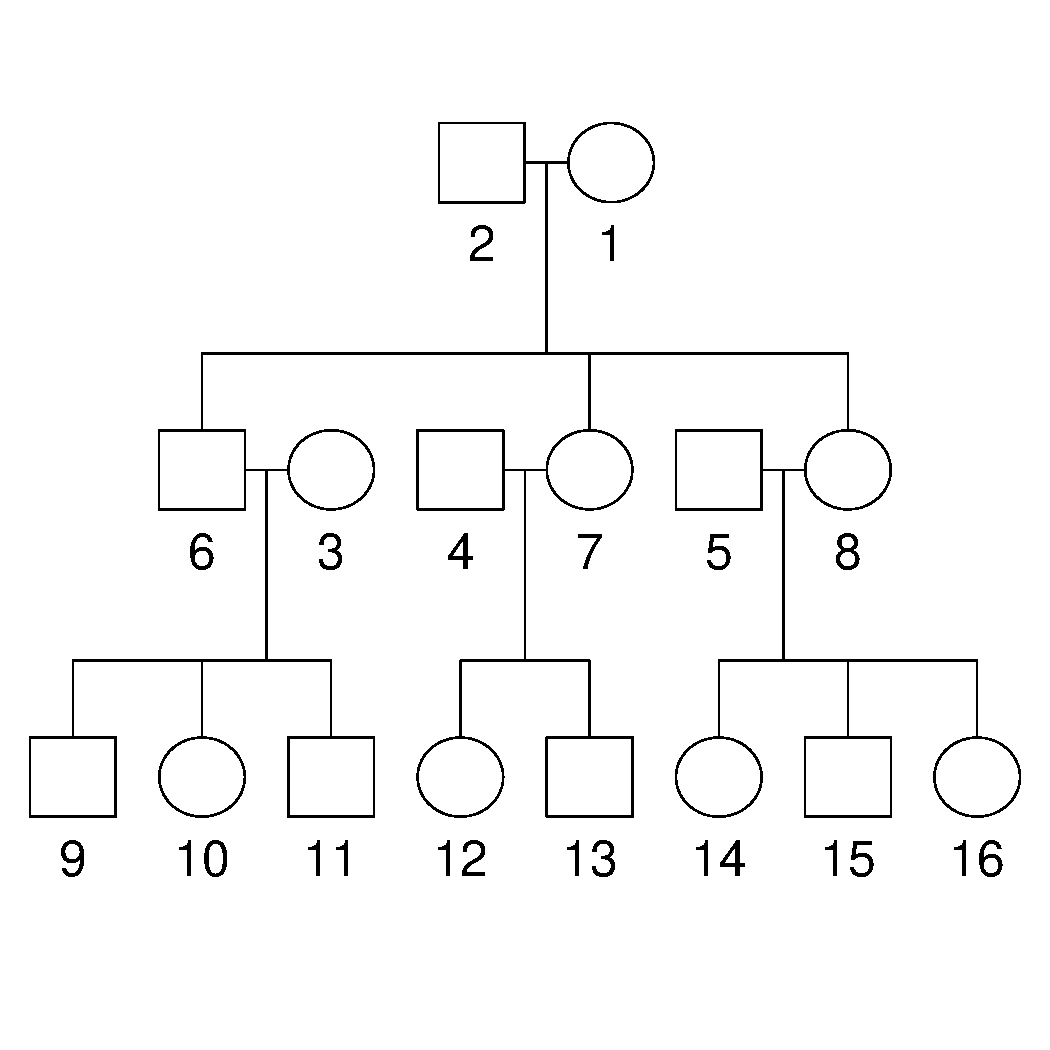
\includegraphics[height=6cm]{../pedigree_16individs.pdf}
\end{figure}
\end{frame}

\begin{frame}
%\frametitle{Step 1: Estimate $\Phi_X$}
\centering
\begin{figure}
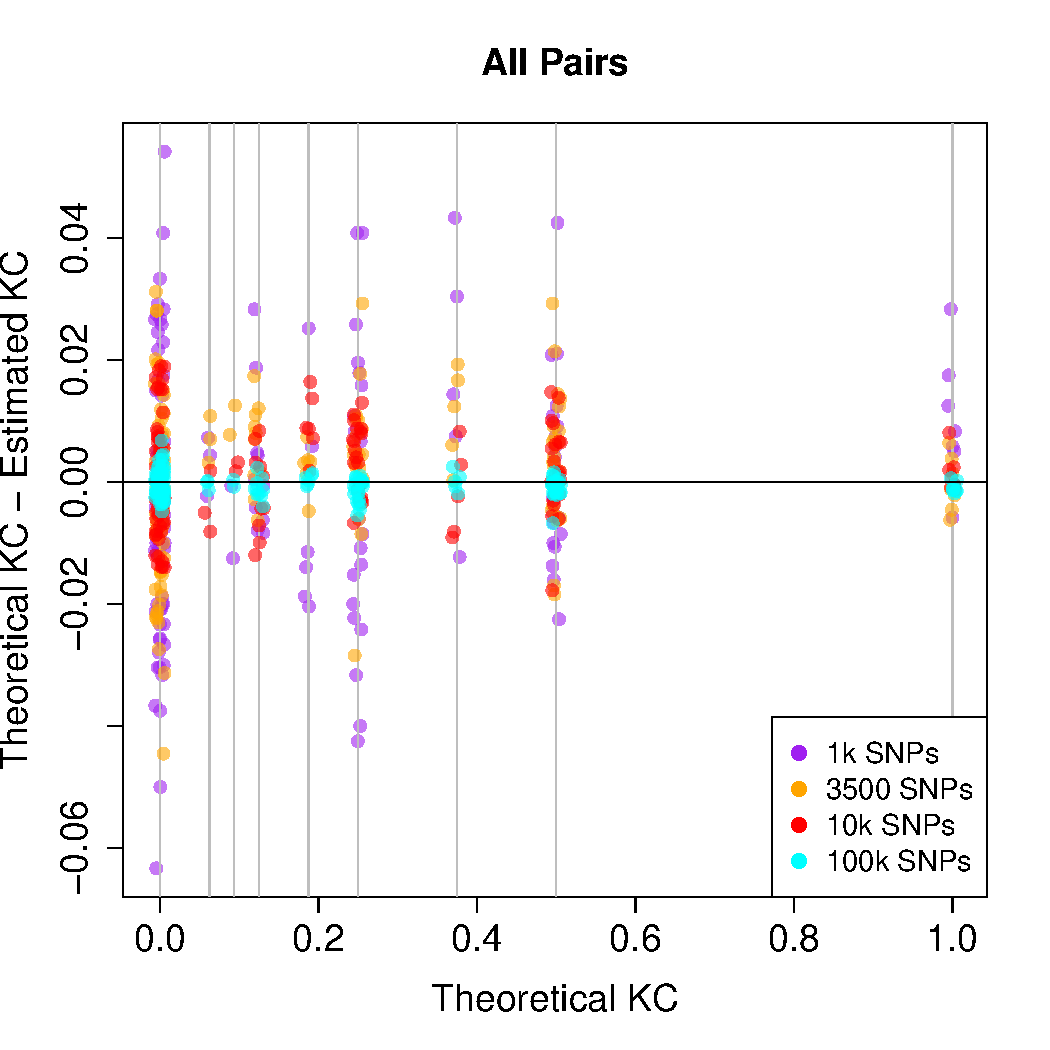
\includegraphics[height=8cm]{../xchr_kc_estimatedVsTrue_horizLines.pdf}
\end{figure}
\end{frame}

\begin{frame}
%\frametitle{Step 1: Estimate $\Phi_X$}
\centering
\begin{figure}
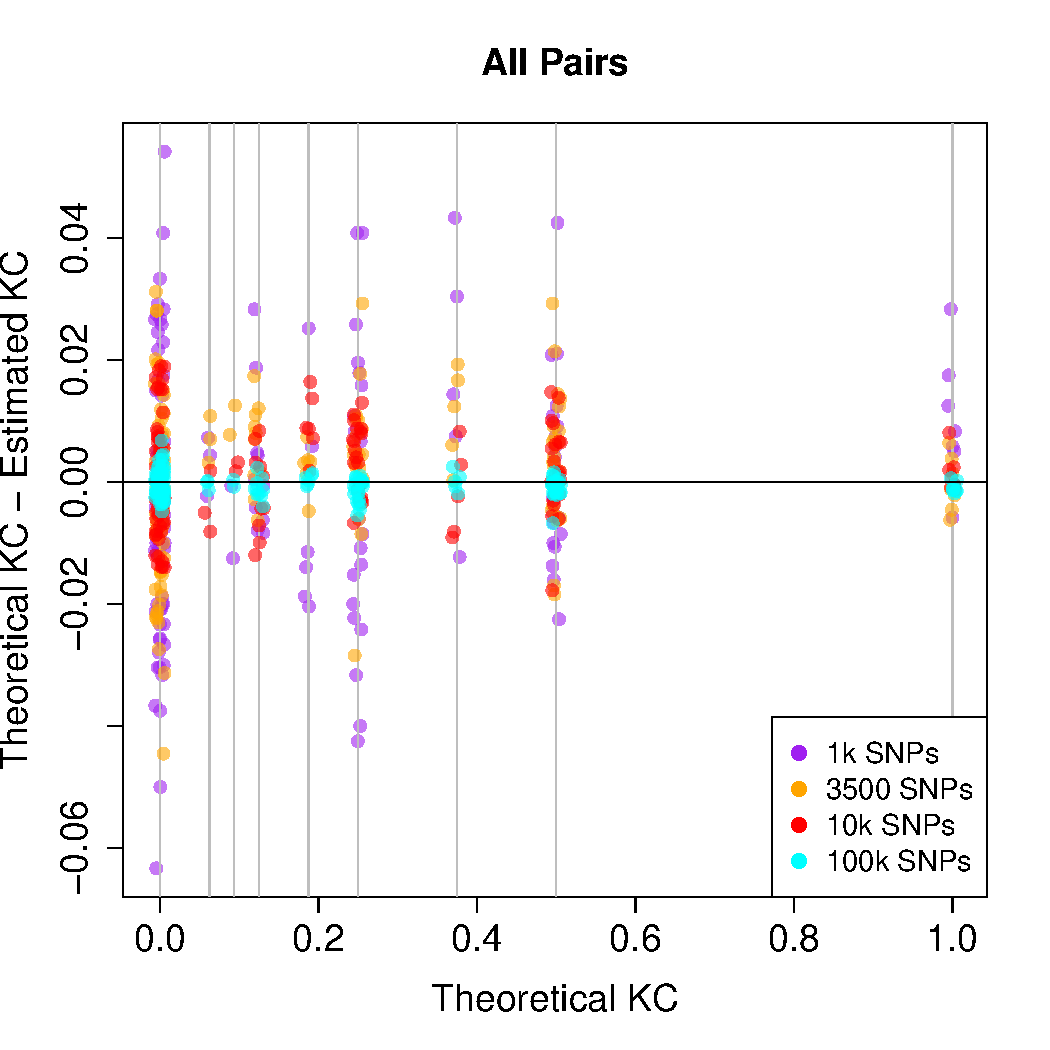
\includegraphics[height=6cm]{../xchr_kc_estimatedVsTrue_horizLines.pdf}
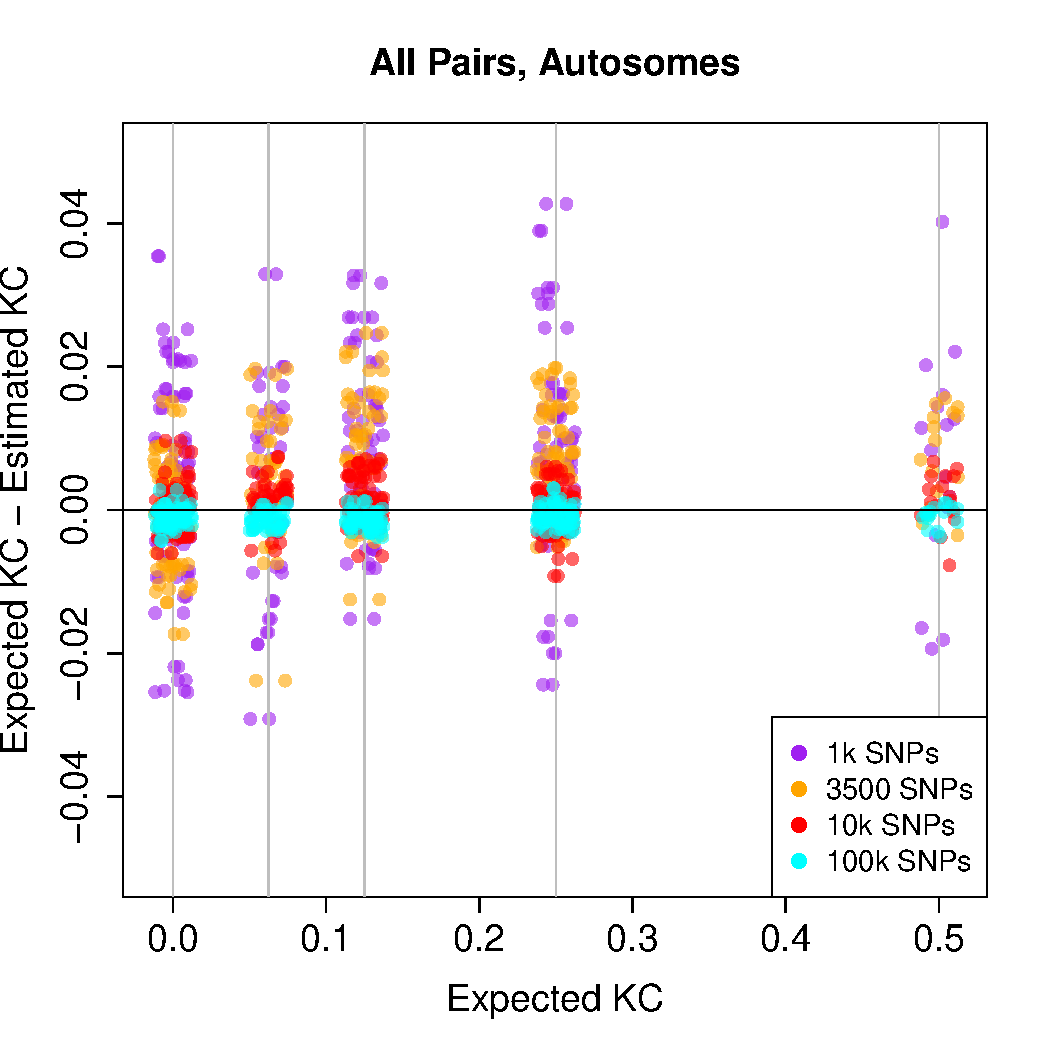
\includegraphics[height=6cm]{../auto_kc_estimatedVsTrue_horizLines.pdf}
\end{figure}
\end{frame}

\begin{frame}
%\frametitle{Step 1: Estimate $\Phi_X$}
\centering
\begin{figure}
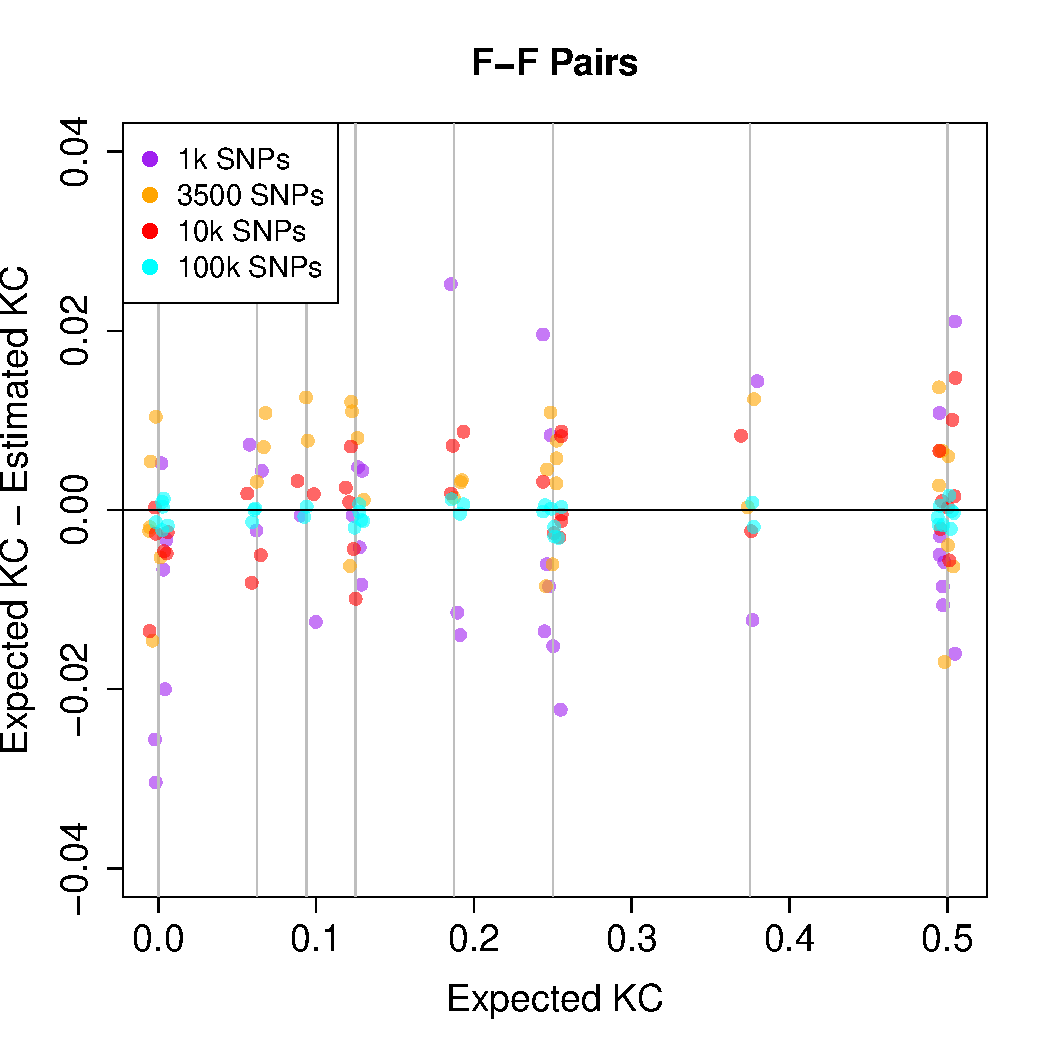
\includegraphics[height=8cm]{../xchr_kc_estimatedVsTrue_FF_horizLines.pdf}
\end{figure}
\end{frame}


\begin{frame}
%\frametitle{Step 1: Estimate $\Phi_X$}
\centering
\begin{figure}
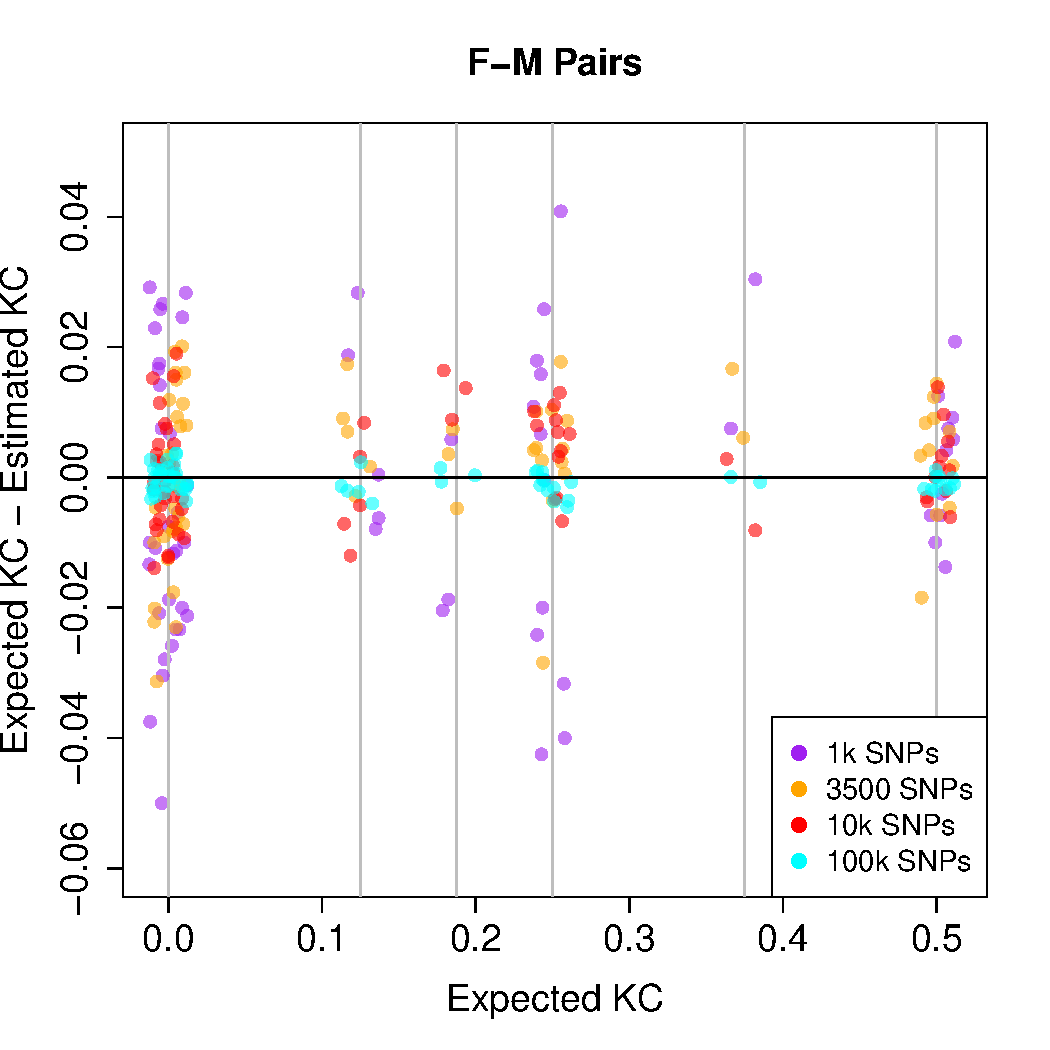
\includegraphics[height=8cm]{../xchr_kc_estimatedVsTrue_FM_horizLines.pdf}
\end{figure}
\end{frame}


\begin{frame}
%\frametitle{Step 1: Estimate $\Phi_X$}
\centering
\begin{figure}
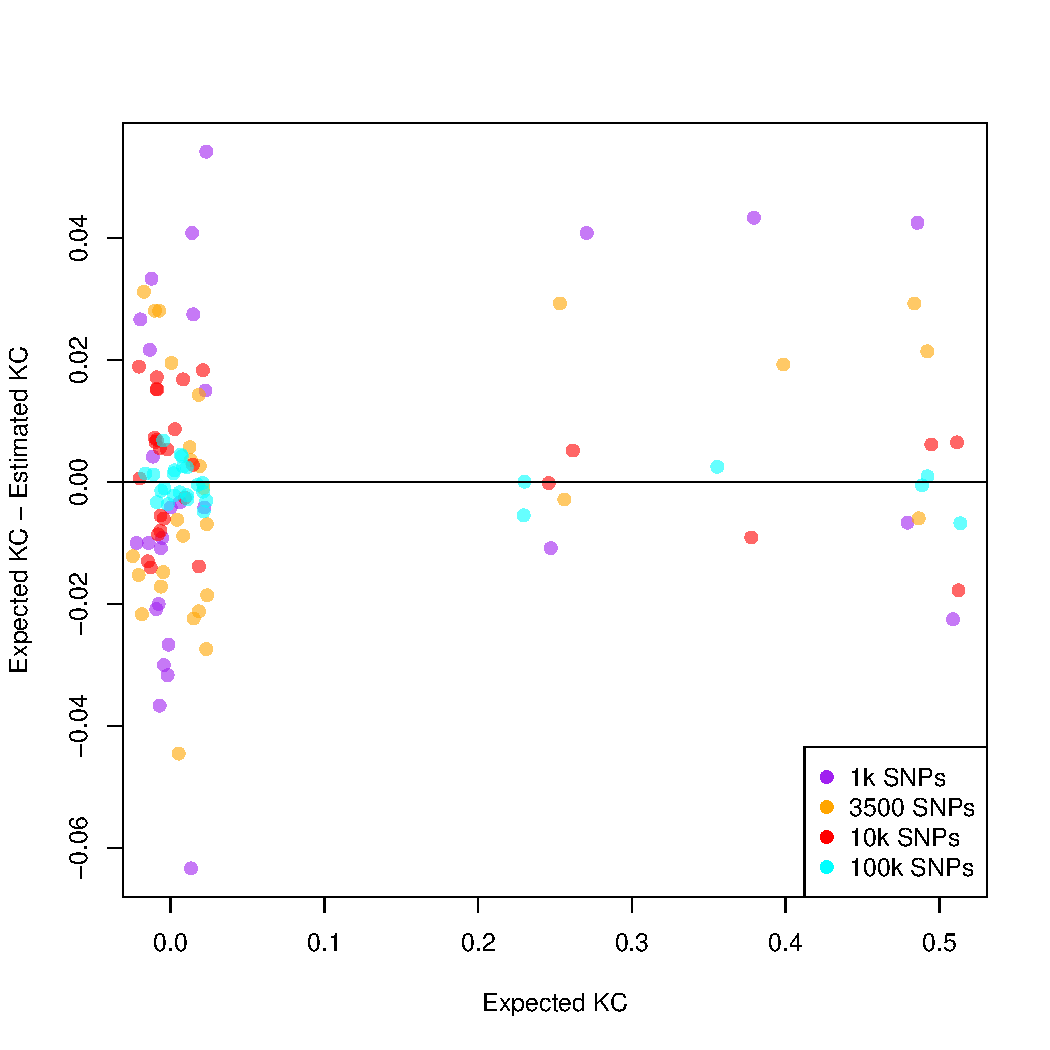
\includegraphics[height=8cm]{../xchr_kc_estimatedVsTrue_MM.pdf}
\end{figure}
\end{frame}

\begin{frame}
%\frametitle{Step 1: Estimate $\Phi_X$}
\begin{itemize}
\item What about samples from an admixed population?
\item We need to determine if we can find `ancestry adjusted' relatedness estimates on the X chromosome.
\begin{itemize}
	\item Using global ancestry, such as PCs estimated on the X. 
	\item Using local ancestry, such as average X chromosome local ancestry. \{\textcolor{blue}{we need X chr local ancestry estimates}\}
\item Or, could we use IBD estimates on the X chromosome from BEAGLE?
\end{itemize}
%\item Or, we can simply include $\mathbf{\hat{\Phi}_X}$ unadjusted for ancestry. 
\end{itemize}
\end{frame}

\begin{frame}
\begin{itemize}
\item We estimated PCs in the SoL subjects using 3,600 LD-pruned X chromosome SNPs and PC-AiR.
\item The unrelated set \texttt{unrelated.pcair.deg4} of 10,272 samples as defined from the autosomes was set, and only study samples (\texttt{subj.plink \& geno.cntl==0}) excluding \texttt{gengrp6.outliers} were projected for a total of 12,747 samples.
\end{itemize}
\end{frame}

\begin{frame}
\centering
\begin{figure}
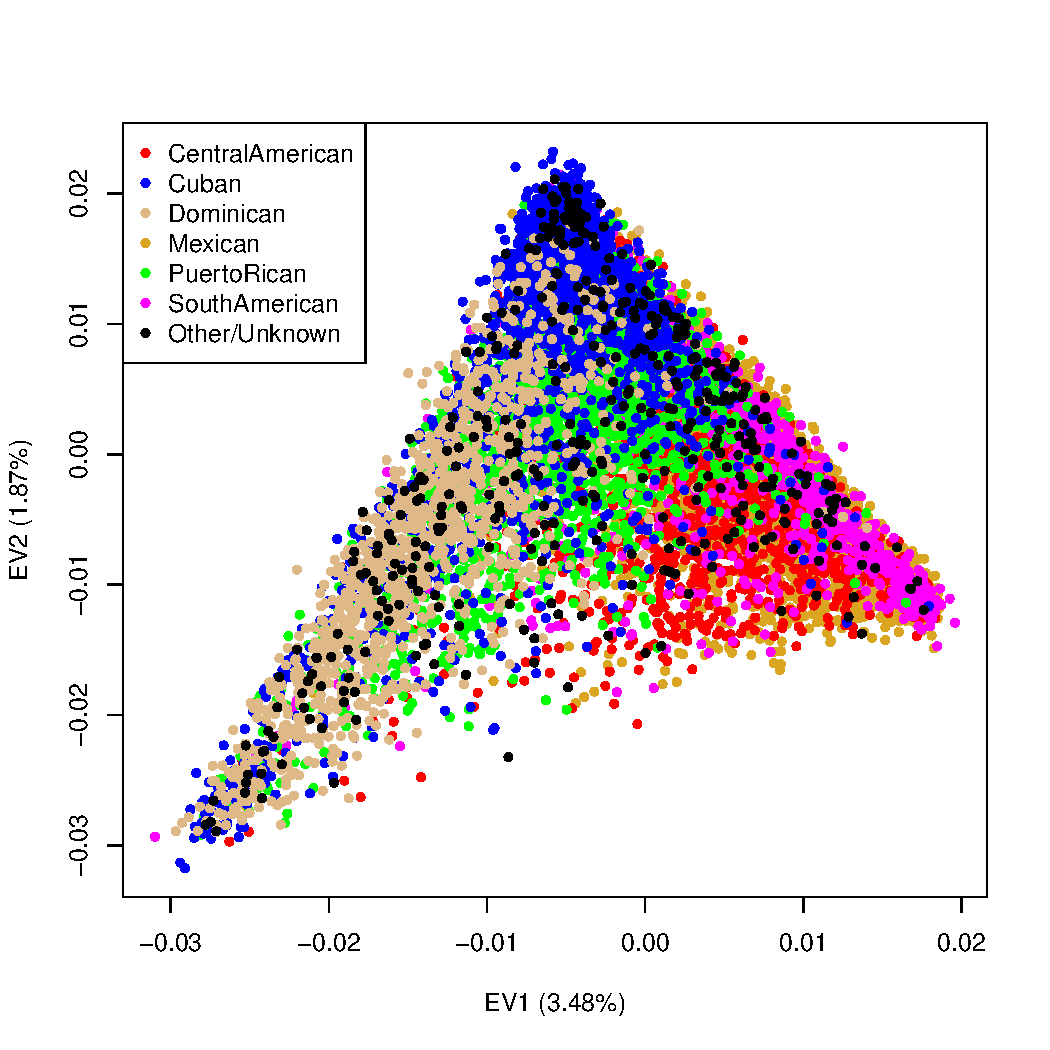
\includegraphics[height=8.5cm]{../pca_x_ev12_col.pdf}
\end{figure}
\end{frame}

\begin{frame}
\centering
\begin{figure}
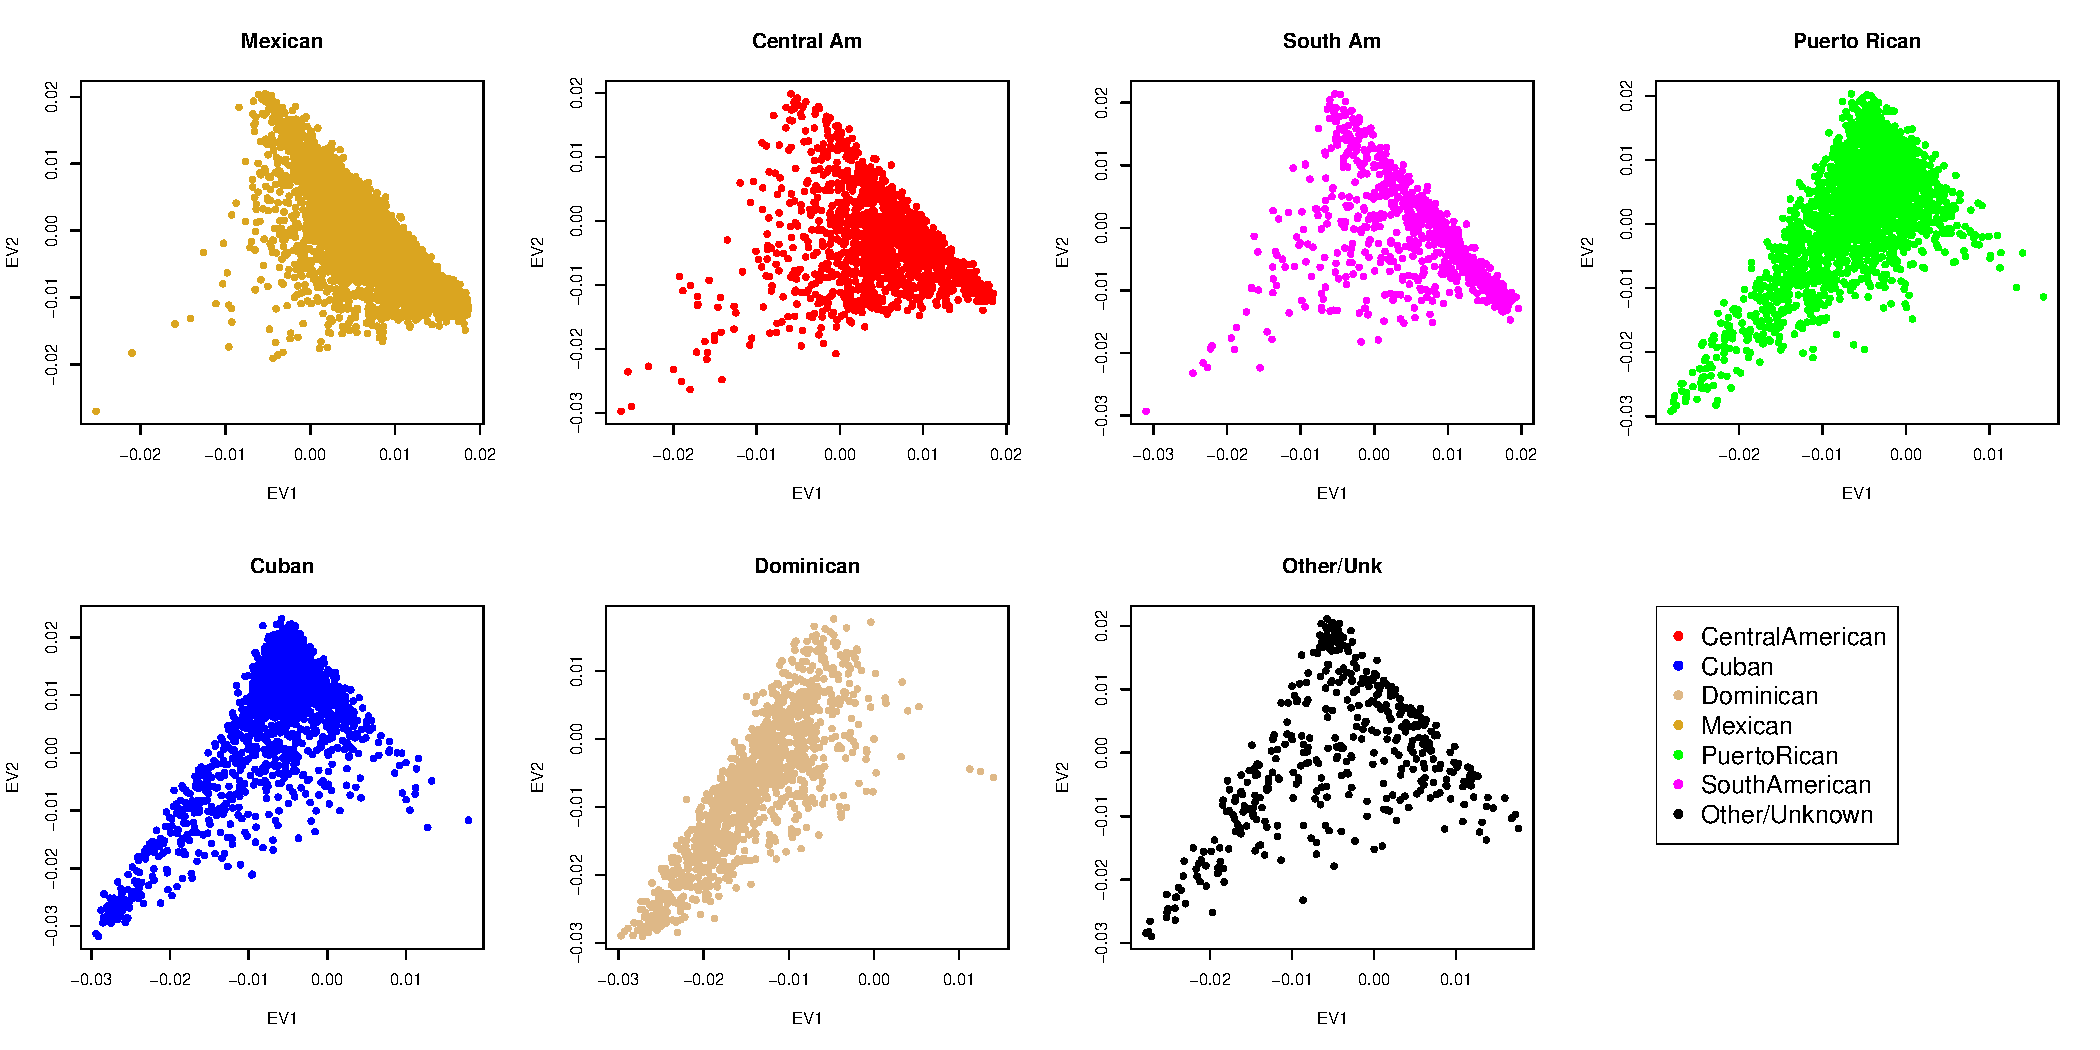
\includegraphics[width=11.5cm]{../pca_x_ev12_eachCol.pdf}
\end{figure}
\end{frame}

\begin{frame}
\centering
\begin{figure}
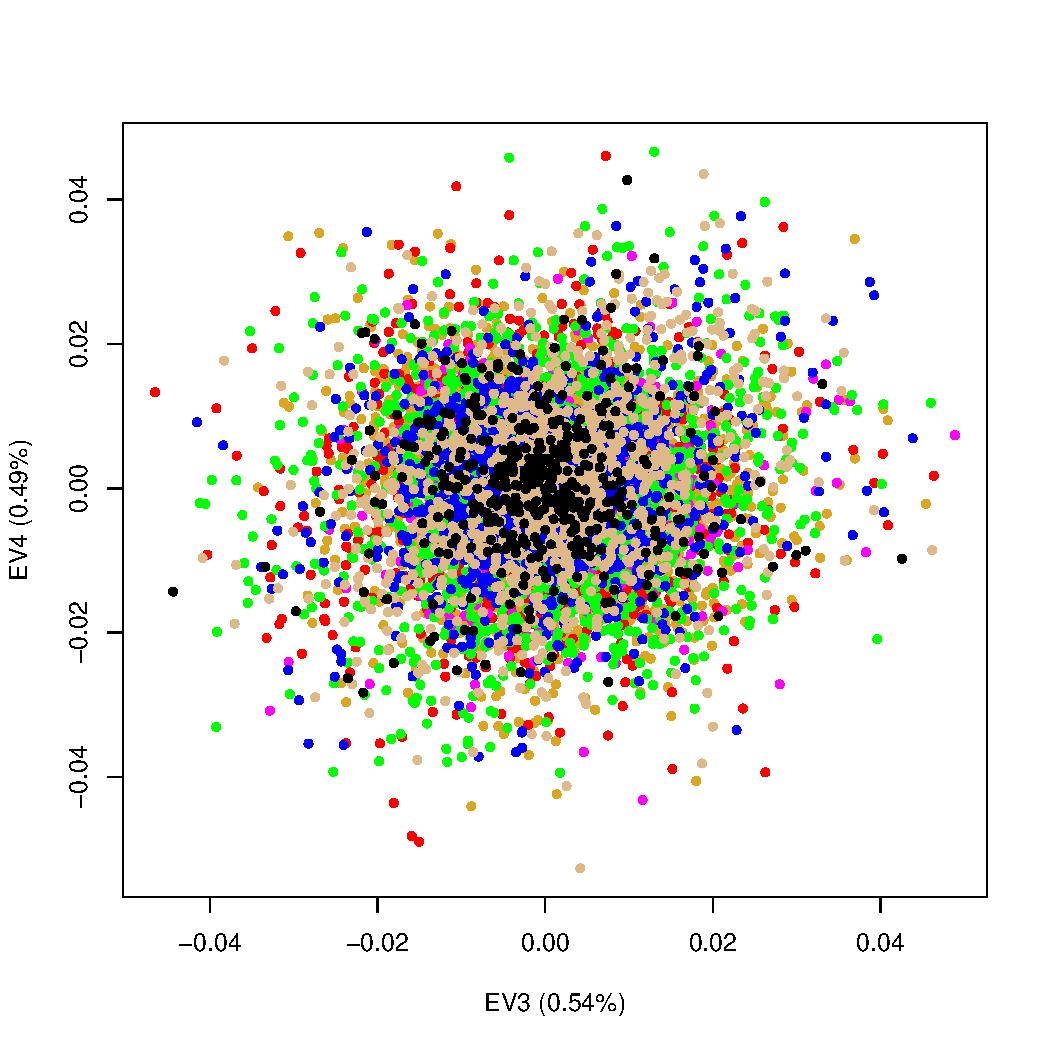
\includegraphics[height=8.5cm]{../pca_x_ev34_col.pdf}
\end{figure}
\end{frame}

\begin{frame}
\centering
\begin{figure}
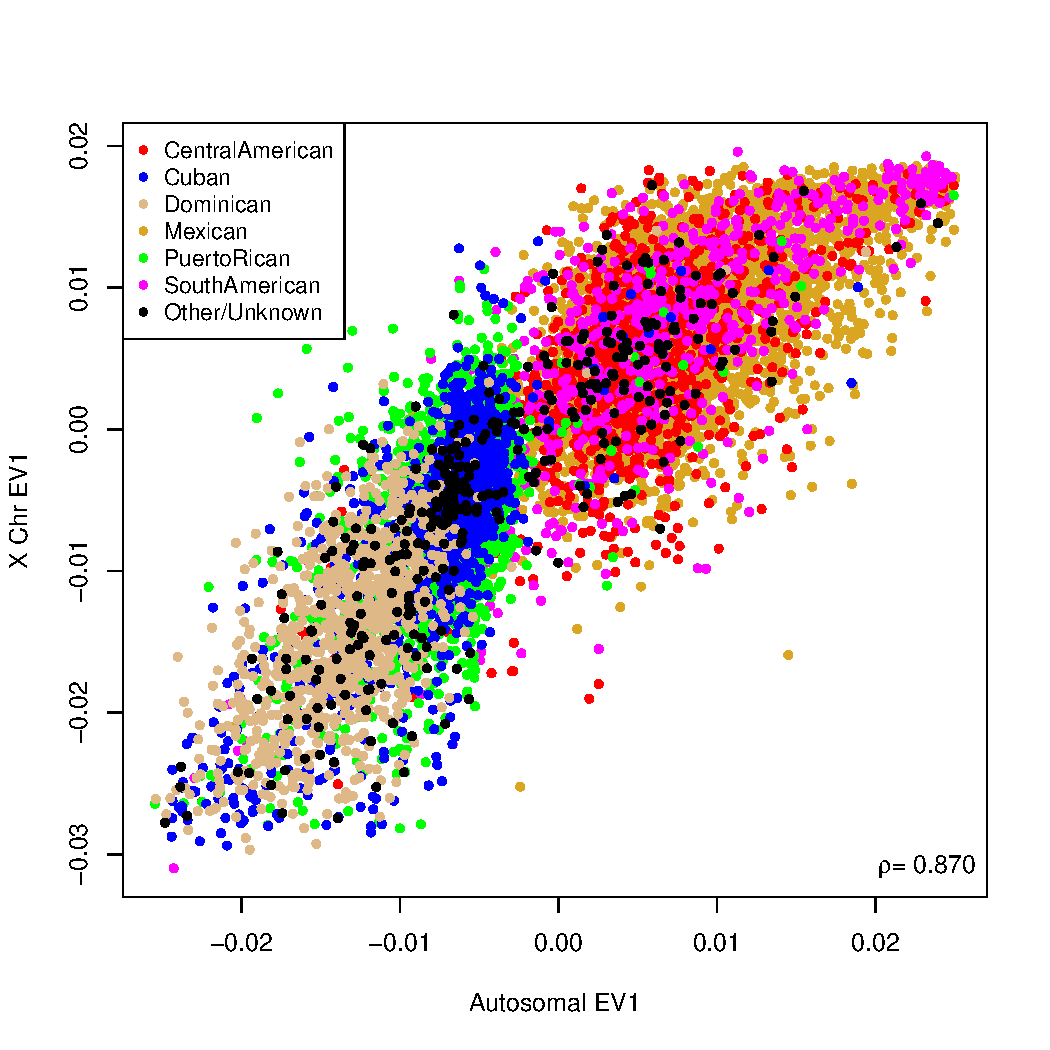
\includegraphics[height=8.5cm]{../pca_x_auto_ev1_col.pdf}
\end{figure}
\end{frame}

\begin{frame}
\centering
\begin{figure}
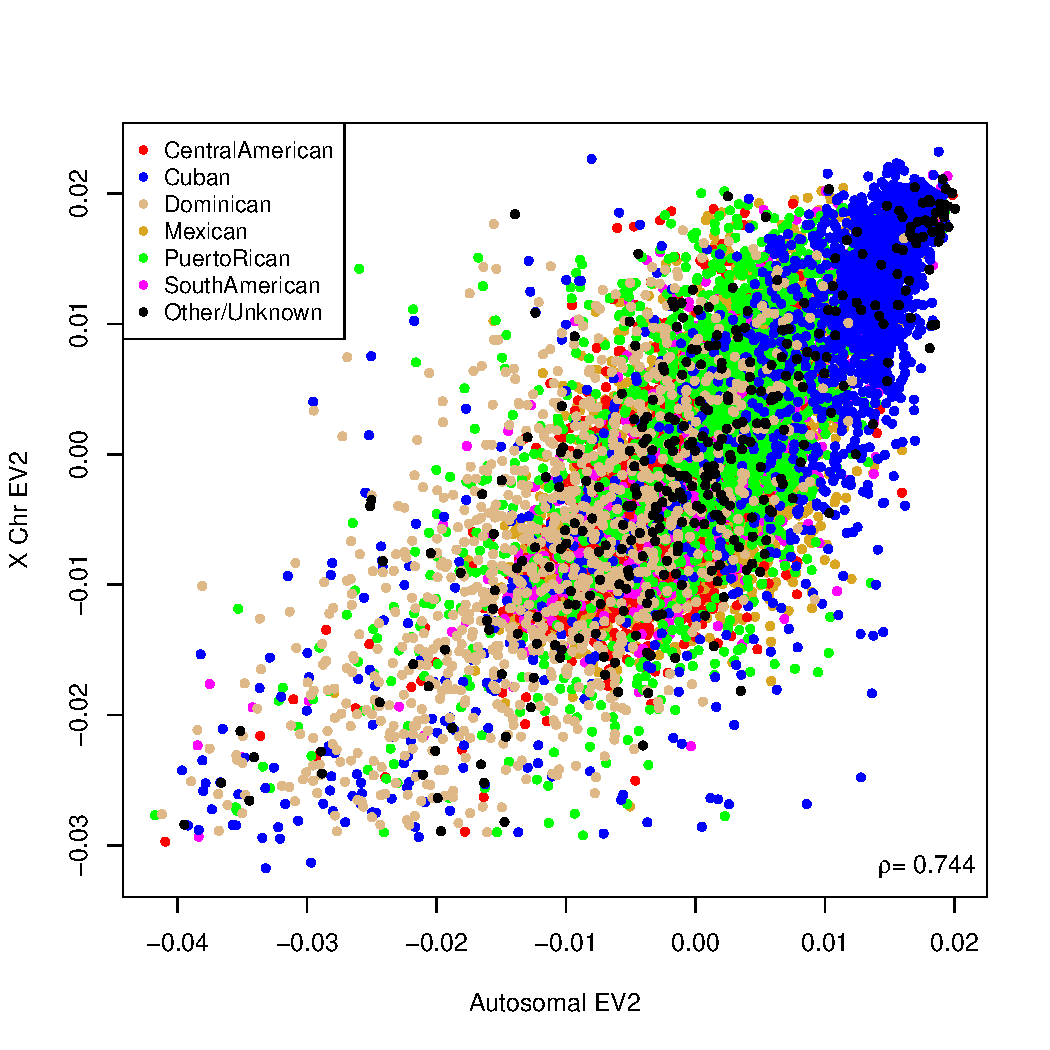
\includegraphics[height=8.5cm]{../pca_x_auto_ev2_col.pdf}
\end{figure}
\end{frame}

\section{Step 2: Determine Covariates}
\begin{frame}%{Step 2: Determine Covariates}
\begin{itemize}
\item What covariates should we include in the model?
\item Should we include PCs calculated across the autosomes?
\item Should we include PCs calculated on the X chromosome? ADMIXTURE estimates from the X chromosome?
Local ancestry estimates averaged across the X chromosome?
\end{itemize}
\end{frame}

\section{Step 3: Fit the Model}
\begin{frame}%{Step 3: Fit the Model}
\begin{itemize}
\item What happens if we simply fit our usual autosomal model when testing X chromosome markers?
\end{itemize}
\end{frame}

\begin{frame}%{Step 3: Fit the Model}
\small
\begin{itemize}
\item Simulate X chromosome genotypes for 8,000 samples = 500 iterations of the 16-person pedigree; 2,500 unrelated + 5,500 relatives.
\item \textit{Note} these samples are from a homogeneous population.
\item Simulate phenotypes that follow the model 
\begin{align*}
Y &= \beta_0 + \beta_1 \mbox{SNP}_X + g_A + g_X  +\epsilon\\
g_A &\sim MVN(0,\sigma^2_A \mathbf{\Phi_A}) \\
g_X &\sim MVN(0, \sigma^2_X \mathbf{\Phi_X}) \\
\epsilon &\sim MVN(0, \mathbb{I})
\end{align*}where $\sigma^2_A=0.3$, $\sigma^2_X=0.8$ and for various $\beta_1$ values.
\item Fit three models:
\begin{align*}
 Y &= \beta_0 + \beta_1 \mbox{SNP}_X + g_A + g_X +\epsilon\\
Y &= \beta_0 + \beta_1 \mbox{SNP}_X + g_X + \epsilon\\
Y &= \beta_0 + \beta_1 \mbox{SNP}_X  + g_A + \epsilon
\end{align*}
\end{itemize}
\end{frame}

\begin{frame}%{Step 3: Fit the Model}
\begin{table}[ht]
\centering
\begin{tabular}{r|ccc}
  \hline
 $\alpha$ & Adj for X + Auto& Adj for X & Adj for Auto \\ 
  \hline
 0.05 & 0.04983 & 0.04867 & 0.07325 \\ 
 0.01 & 0.00931 & 0.00913 & 0.02080 \\ 
 0.005 & 0.00494 & 0.00534 & 0.01095 \\ 
 0.001 & 0.00094 & 0.00102 & 0.00191 \\ 
   \hline
\end{tabular}
\caption{Type I error rate as calculated from 22,000 simulation iterations where $\beta_1$=0.}
\end{table}
\end{frame}

\begin{frame}%{Step 3: Fit the Model}
\begin{itemize}
\item When only adjusting for autosomal effects, no type I error CIs include the $\alpha$ under consideration.
\end{itemize}
\begin{table}[ht]
\centering
\begin{tabular}{r|cc}
  \hline
  $\alpha$ & Estimate & 95\% CI \\ 
  \hline
 0.05 & 0.07325 & (0.07040, 0.07610) \\ 
 0.01 & 0.02080 & (0.01949,  0.02210) \\ 
 0.005 & 0.01095 & (0.01003,  0.01188) \\ 
 0.001 & 0.00191 & (0.00150,  0.00233) \\ 
   \hline
\end{tabular}
\caption{Estimate and 95\% CI for type I error rate as calculated from 22,000 simulations where $\beta_1$=0 and fitting the model $Y = \beta_0 + \beta_1 \mbox{SNP}_X + g_A + \epsilon$.}
\end{table}
\end{frame}

\begin{frame}
\begin{itemize}
\item For each $\alpha$ value ranging from 1e-04 to 1, and 7,500 simulation iterations, we calculate the 
true and false positive rate for each model.
\end{itemize}
\begin{figure}
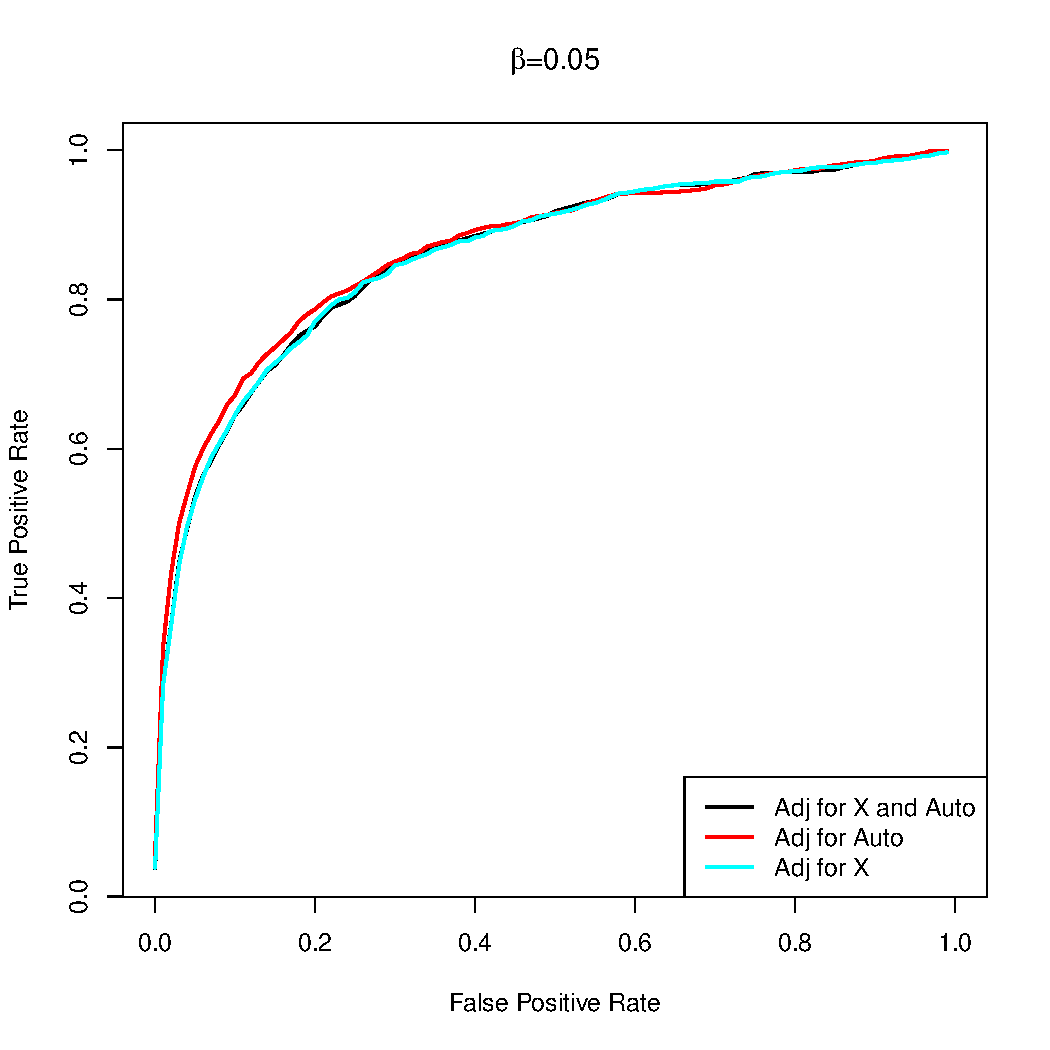
\includegraphics[height=6.5cm]{../power_3models_beta05.pdf}
\end{figure}
\end{frame}

\begin{frame}
\begin{figure}
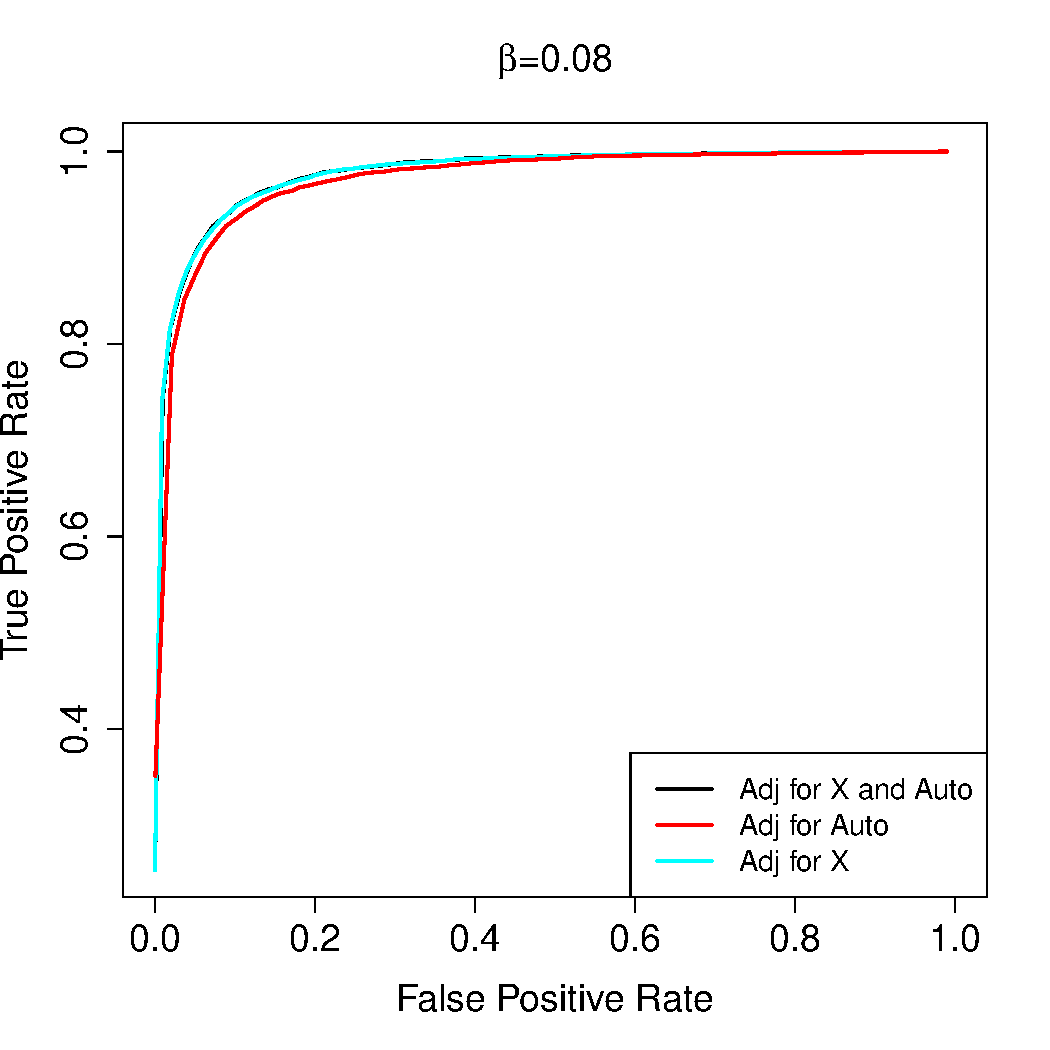
\includegraphics[height=6.5cm]{../power_3models_beta08.pdf}
\end{figure}
\end{frame}

%%%%%%%% SUPPLEMENTARY SLIDES 
\begin{frame}
\Large
\centering
Supplementary Slides
\end{frame}

\begin{frame}
\begin{align*}
cov(\mbox{F,M})&=\mathbb{E}(\mbox{F,M})-\mathbb{E}(\mbox{F})\mathbb{E}(\mbox{M})\\
&=\mathbb{E}(\mbox{FM}|\mbox{IBD})\Phi_X +\mathbb{E}(\mbox{FM}|\mbox{not IBD})(1-\Phi_X) -(2p)^2 \\
&=[4p^2 + 4p(1-p)]\Phi_X + [4p^3 + 4p^2(1-p)](1-\Phi_X) -4p^2 \\
&= 4p(1-p)\Phi_X
\end{align*}
\end{frame}


\begin{frame}{Type I Error CIs}
\begin{table}[ht]
\centering
\begin{tabular}{r|cc}
  \hline
  $\alpha$ & Estimate & 95\% CI \\ 
  \hline
 0.05 & 0.04867 & (0.04582, 0.05152) \\ 
 0.01 & 0.00913 & (0.00783, 0.01043) \\ 
 0.005 & 0.00534 & (0.00442, 0.00627) \\ 
 0.001 & 0.00102 & (0.00061, 0.00144) \\ 
   \hline
\end{tabular}
\caption{Estimate and 95\% CI for type I error rate as calculated from 22,000 simulations where $\beta_1$=0 and fitting the model $Y = \beta_0 + \beta_1 \mbox{SNP}_X + g_X + \epsilon$.}
\end{table}
\end{frame}

\begin{frame}{Type I Error CIs}
\begin{table}[ht]
\centering
\begin{tabular}{r|cc}
  \hline
  $\alpha$ & Estimate & 95\% CI \\ 
  \hline
 0.05 & 0.04983 & (0.04698, 0.05268) \\ 
0.01 & 0.00931 & (0.00801, 0.01061) \\ 
0.005 & 0.00494 & (0.00402, 0.00587) \\ 
 0.001 & 0.00094 & (0.00052, 0.00135) \\ 
   \hline
\end{tabular}
\caption{Estimate and 95\% CI for type I error rate as calculated from 22,000 simulations where $\beta_1$=0 and fitting the model $Y = \beta_0 + \beta_1 \mbox{SNP}_X + g_A + g_X + \epsilon$.}
\end{table}
\end{frame}

\begin{frame}
\centering
\begin{figure}
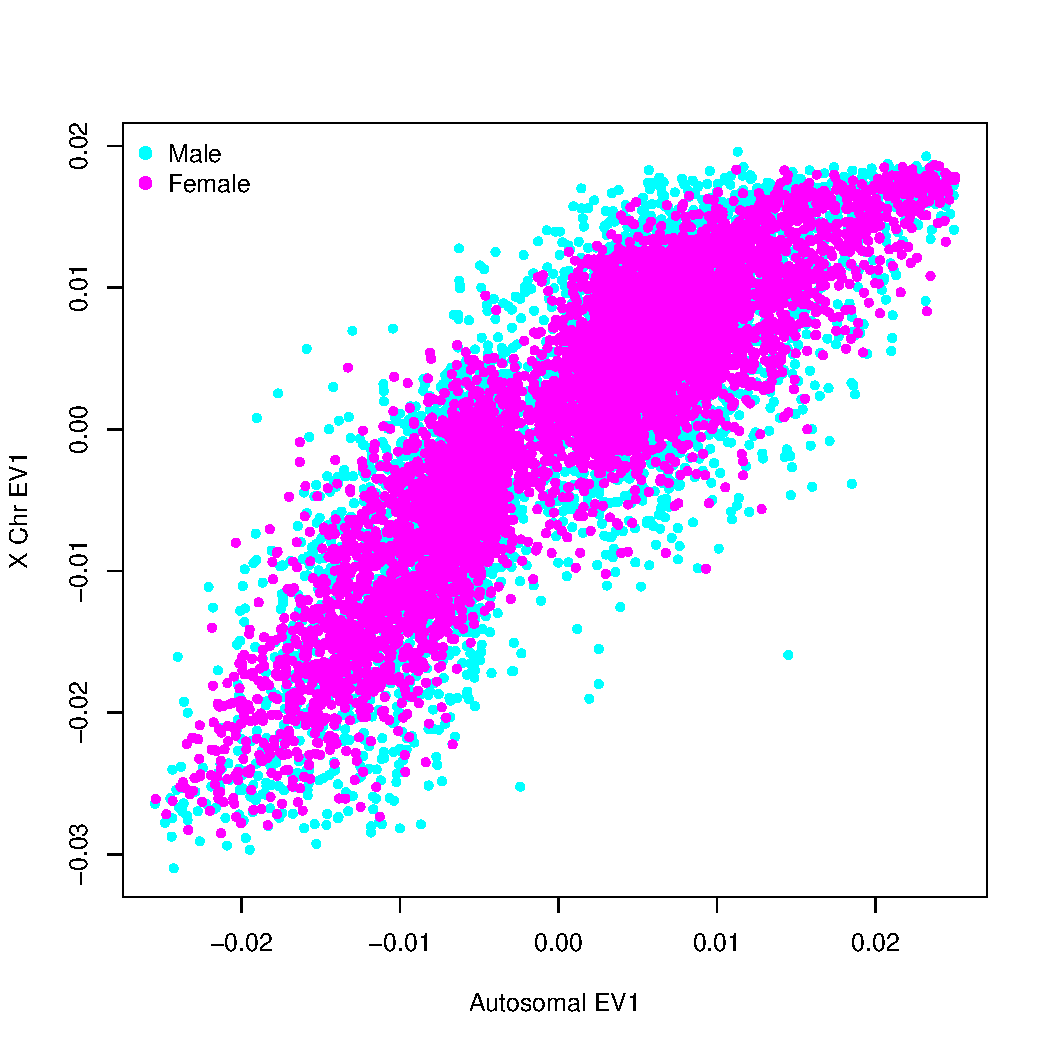
\includegraphics[height=8.5cm]{../pca_x_auto_ev1_sexCol.pdf}
\end{figure}
\end{frame}


\end{document}


